\documentclass{article}

\usepackage{amsmath, amssymb}
\usepackage[utf8]{inputenc}
\usepackage{geometry}
\usepackage{tikz}
\usetikzlibrary{arrows.meta}
\usetikzlibrary{fit}
\usetikzlibrary{positioning}

\begin{document}
\section{List Of Models}
\subsection{Infinite Words}
\begin{itemize}
	\item DBA
	\item NBA
	\item GBA
	\item Rabin automaton
	\item Muller automaton
	\item Parity automaton
	\item E automaton
	\item A automaton
	\item coBA
	\item weak BA
	\item Staiger-Wagner automaton
	\item ABA
	\item LTL
	\item S1S
	\item $\exists$S1S
	\item S1S\textsubscript{0}
\end{itemize}

\subsection{Finite Trees}
\begin{itemize}
	\item DTA
	\item NTA
	\item $\downarrow$DTA
	\item $\downarrow$NTA
	\item DUTA
	\item NUTA
	\item DTD
	\item deterministic EDTD
	\item single-type EDTD
	\item EDTD
	\item Relax NG
	\item FO
	\item MSO
	\item Regular expressions
	\item DTWA
	\item TWA
\end{itemize}

\subsection{Infinite Trees}
\begin{itemize}
	\item BTA
	\item Muller TA
	\item Parity TA
	\item DMTA
	\item S2S (MSO / WMSO)
	\item S2S\textsubscript{0} (MSO / WMSO)
\end{itemize}

\section{List Of Games}
\begin{itemize}
	\item Büchi
	\item Staiger-Wagner
	\item weak Parity
	\item Reachability
	\item Safety
	\item Muller
	\item Parity
	\item Rabin
	\item Streett
	\item Gale-Stewart
	\item Wadge
\end{itemize}

\newpage

\section{Infinite Word Models}
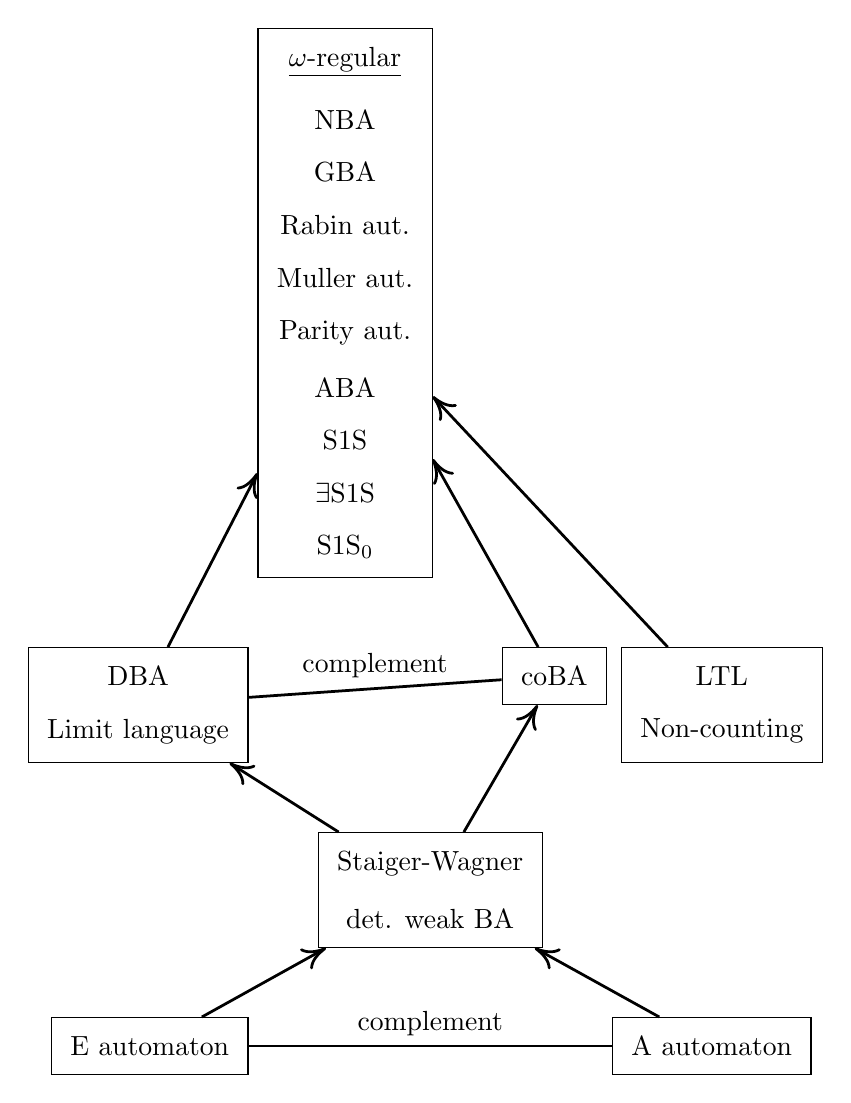
\begin{tikzpicture}
  \node (ireg) {\underline{$\omega$-regular}};
  \node (iNBA) [below=5pt of ireg] {NBA};
  \node (iGBA) [below=5pt of iNBA] {GBA};
  \node (iRabin) [below=5pt of iGBA] {Rabin aut.};
  \node (iMuller) [below=5pt of iRabin] {Muller aut.};
  \node (iParity) [below=5pt of iMuller] {Parity aut.};
  \node (iABA) [below=5pt of iParity] {ABA};
  \node (iS1S) [below=5pt of iABA] {S1S};
  \node (iES1S) [below=5pt of iS1S] {$\exists$S1S};
  \node (iS1S0) [below=5pt of iES1S] {S1S\textsubscript{0}};
  \node [draw, fit={(ireg) (iNBA) (iGBA) (iRabin) (iMuller) (iParity) (iABA) (iS1S) (iES1S) (iS1S0)}] (c1) {};
  
  \node (iDBA) [below left=of c1] {DBA};
  \node (ilimit) [below=5pt of iDBA] {Limit language};
  \node [draw, fit={(iDBA) (ilimit)}] (c2) {};
  
  \node (icoBA) [below right=of c1] {coBA};
  \node [draw, fit={(icoBA)}] (c3) {};
  
  \node (iSW) [below right=of c2] {Staiger-Wagner};
  \node (iweakBA) [below=5pt of iSW] {det. weak BA};
  \node [draw, fit={(iSW) (iweakBA)}] (c4) {};
  
  \node (iLTL) [right=of c3] {LTL};
  \node (inonc) [below=5pt of iLTL] {Non-counting};
  \node [draw, fit={(iLTL) (inonc)}] (c5) {};
  
  \node (iEA) [below left=of c4] {E automaton};
  \node [draw, fit={(iEA)}] (c6) {};
  
  \node (iAA) [below right=of c4] {A automaton};
  \node [draw, fit={(iAA)}] (c7) {};
  
   \draw [-{>[length=3mm,width=3mm]}, line width=1pt] (c2) -- (c1);
   \draw [-{>[length=3mm,width=3mm]}, line width=1pt] (c3) -- (c1);
   \draw [-{>[length=3mm,width=3mm]}, line width=1pt] (c5) -- (c1);
   \draw [-{>[length=3mm,width=3mm]}, line width=1pt] (c4) -- (c2);
   \draw [-{>[length=3mm,width=3mm]}, line width=1pt] (c4) -- (c3);
   \draw [-{>[length=3mm,width=3mm]}, line width=1pt] (c6) -- (c4);
   \draw [-{>[length=3mm,width=3mm]}, line width=1pt] (c7) -- (c4);
   \draw [-, line width=1pt] (c2) -- node [midway,above] {complement} (c3);
   \draw [-, line width=1pt] (c6) -- node [midway,above] {complement} (c7);
\end{tikzpicture}

\subsection{Class Inclusions}
\begin{itemize}
	\item E aut. $\subseteq$ Staiger-Wagner \\
		\textbf{Proof}: SWA with $\mathcal{F} = \{ Q' \subseteq Q \mid F \cap Q' \neq \emptyset \}$.
    \item A. aut. $\subseteq$ Staiger-Wagner \\
    	\textbf{Proof}: SW closed under complement,
    \item Staiger-Wagner $\subseteq$ DBA / coBA \\
    	\textbf{Proof}: $\mathcal{A}$ SWA $\Rightarrow$ $\mathcal{A}' = (Q \times 2^Q, \Sigma, (q_0, \emptyset), \delta', F')$ \\
    	Collect all visited states and accept if that set stays in $\mathcal{F}$.
    \item DBA $\subseteq$ NBA \\
    	trivial
    \item coBA $\subseteq$ NBA \\
    	\textbf{Proof}: NBA closed under complement.
    \item LTL $\subseteq$ NBA \\
    	\textbf{Proof}: \ref{} %TODO 6
    \item LTL $\subseteq$ ABA \\
    	\textbf{Proof}: \ref{} %TODO 21-22
\end{itemize}

\subsection{Class Exclusions}
\begin{itemize}
	\item E aut. $\not\subseteq$ A aut. \\
		\textbf{Example}: $(a+b)^* a (a+b)^\omega$ \\
    	\textbf{Proof}: \ref{} %TODO
	\item A aut. $\not\subseteq$ E aut. \\
		\textbf{Example}: $\{a^\omega\}$ \\
    	\textbf{Proof}: \ref{} %TODO
	\item DBA $\not\subseteq$ coBA \\
		\textbf{Example}: $(a^*b)^\omega$ \\
    	\textbf{Proof}: \ref{} %TODO
	\item coBA $\not\subseteq$ DBA \\
		\textbf{Example}: $(a+b)^* a^\omega$ \\
    	\textbf{Proof}: \ref{} %TODO
	\item LTL $\not\subseteq$ NBA \\
		\textbf{Example}: $((a+b) a)^\omega$ \\
    	\textbf{Proof}: \ref{} %TODO
\end{itemize}

\subsection{Class Equalities}
\subsubsection{NBA}
\begin{itemize}
	\item NBA $\Rightarrow$ $\omega$-regular \\
    	\textbf{Proof}: \ref{} %TODO F3
	\item $\omega$-regular $\Rightarrow$ NBA \\
    	\textbf{Proof}: \ref{} %TODO F3
    \item NBA $\Rightarrow$ $\exists$S1S \\
    	\textbf{Proof}: \ref{} %TODO F9
    \item S1S $\Rightarrow$ S1S\textsubscript{0} \\
    	\textbf{Proof}: \ref{} %TODO F9
    \item S1S\textsubscript{0} $\Rightarrow$ NBA \\
    	\textbf{Proof}: \ref{} %TODO F10
    \item Det. Muller $\Rightarrow$ NBA \\
    	\textbf{Proof}: NBA with $L(\mathcal{A}) = \bigcup\limits_{F \in \mathcal{F}} \left( \bigcap\limits_{q \in F} L(\mathcal{A}_q) \cap \bigcap\limits_{q \notin F} \overline{L(\mathcal{A}_q)} \right)$ where $\mathcal{A}_q$ is $\mathcal{A}$ starting in $q$.
    \item NBA $\Rightarrow$ det. Muller \\
    	\textbf{Proof}: \ref{} %TODO F12
   	\item (det.) Muller $\Rightarrow$ (det.) Parity \\
   		\textbf{Proof}: \ref{} %TODO F14
   	\item ABA $\Rightarrow$ NBA \\
   		\textbf{Proof}: \ref{} %TODO F23
\end{itemize}

\subsubsection{LTL}
LTL $\Leftrightarrow$ Non-counting \\
No proof. Remarks in F8.

\subsubsection{SW}
Staiger-Wagner $\Leftrightarrow$ det. weak BA \\
\textbf{Proof}: \ref{} %TODO F18

\subsection{Closures}
\subsubsection{NBA}
\begin{itemize}
	\item Closed under union \\
    	\textbf{Proof}: \ref{} %TODO F3
    \item Closed under intersection \\
    	\textbf{Proof}: \ref{} %TODO F3
    \item Closed under complement \\
    	\textbf{Proof}: \ref{} %TODO F4
\end{itemize}

\subsubsection{DBA}
\begin{itemize}
	\item Not closed under complement (inf. many $a$ $\leftrightarrow$ fin. many $a$)
\end{itemize}

\subsubsection{SW}
\begin{itemize}
	\item Closed under union \\
    	\textbf{Proof}: \ref{} %TODO F18
    \item Closed under intersection \\
    	\textbf{Proof}: \ref{} %TODO F18
    \item Closed under complement \\
    	\textbf{Proof}: \ref{} %TODO F18
\end{itemize}

\subsection{Characterizations}
\begin{itemize}
	\item Parity conditions are directly convertible to Rabin chain conditions and vice-versa. \\
		\textbf{Proof}: Assign priorities in ascending order; $E_k \rightarrow 0$, $F_k \setminus E_k \rightarrow 1$, $E_{k-1} \setminus F_k \rightarrow 2$ \dots
	\item $U$ is $\omega$-regular iff $U$ is a Boolean combination of DBA-languages \\
		\textbf{Proof}: NBAs are closed under Boolean operations. %TODO other direction
	\item $U$ is DBA-recog. iff $U = \text{lim}(L)$ for some regular $L \subseteq \Sigma^*$. \\
		\textbf{Proof}: \ref{} %TODO F2
	\item $U$ is E-recog. iff $U = L \cdot \Sigma^*$ for some regular $L \subseteq \Sigma^*$. \\
		\textbf{Proof}: \ref{} %TODO F16
	\item Landweber's theorem \\
		\textbf{Proof}: \ref{} %TODO F16-F18
	\item DBA $\cap$ coBA $\Rightarrow$ SW \\
		\textbf{Proof}: \ref{} %TODO F18
\end{itemize}

\subsection{Duality}
\begin{itemize}
	\item $U$ is A-recog. iff $\Sigma^\omega \setminus U$ is E-recog. \\
		\textbf{Proof}: \ref{} %TODO F16
	\item $U$ is coBA-recog. iff $\Sigma^\omega \setminus U$ is DBA-recog. \\
		\textbf{Proof}: \ref{} %TODO F16
\end{itemize}

\subsection{Problems / Complexity}
\begin{itemize}
	\item Emptiness problem for NBAs is decidable in poly. time. \\
    	\textbf{Proof}: \ref{} %TODO F4
    \item Emptiness problem for ABAs is PSPACE-complete. \\
    	No proof. Remarks in F23.
    \item Membership problem for ABAs is decidable in poly. time. \\
    	%TODO F23;  infinite games?
\end{itemize}


\newpage

\section{Finite Tree Models}
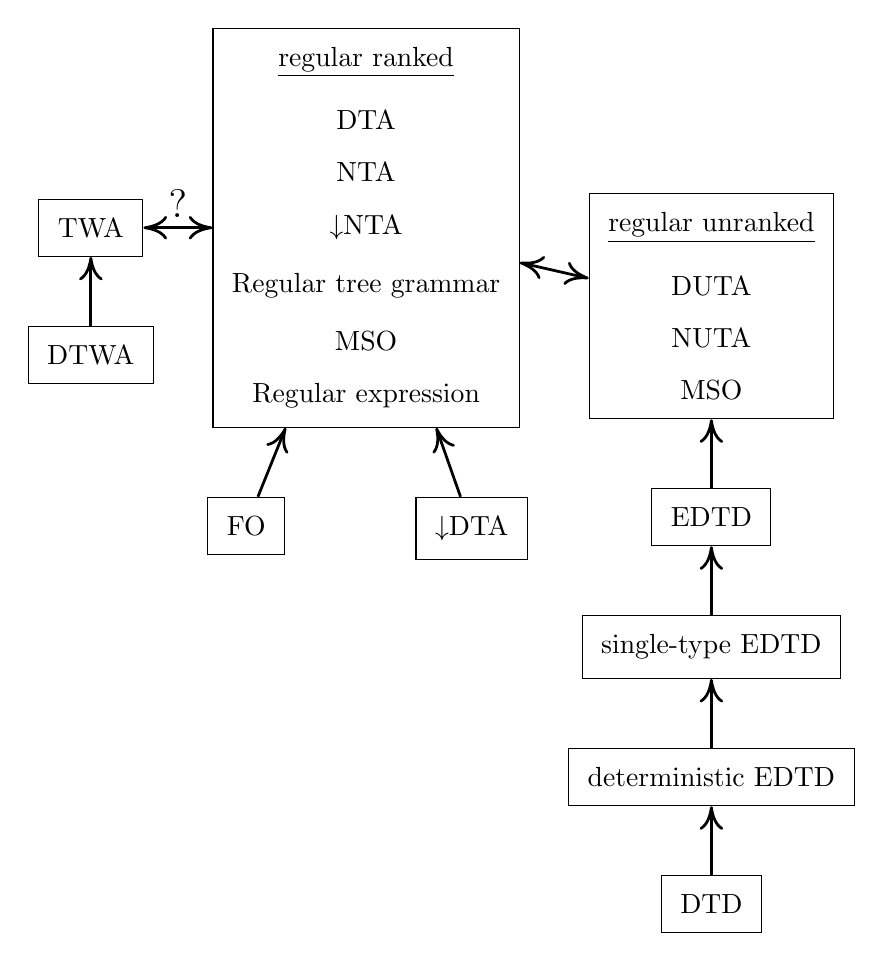
\begin{tikzpicture}
  \node (ireg) {\underline{regular ranked}};
  \node (iDTA) [below=5pt of ireg] {DTA};
  \node (iNTA) [below=5pt of iDTA] {NTA};
  \node (idNTA) [below=5pt of iNTA] {$\downarrow$NTA};
  \node (iRegGram) [below=5pt of idNTA] {Regular tree grammar};
  \node (iMSO) [below=5pt of iRegGram] {MSO};
  \node (iRegex) [below=5pt of iMSO] {Regular expression};
  \node [draw, fit={(ireg) (iDTA) (iNTA) (idNTA) (iRegGram) (iMSO) (iRegex)}] (c1) {};
  
  \node (iregu) [right=of c1] {\underline{regular unranked}};
  \node (iDUTA) [below=5pt of iregu] {DUTA};
  \node (iNUTA) [below=5pt of iDUTA] {NUTA};
  \node (iMSOu) [below=5pt of iNUTA] {MSO};
  \node [draw, fit={(iregu) (iDUTA) (iNUTA) (iMSOu)}] (c2) {};
  
  \node (idDTA) [below right=1cm and -1.2cm of c1] {$\downarrow$DTA};
  \node [draw, fit={(idDTA)}] (c3) {};
  
  \node (iFO) [below left=1cm and -0.8cm of c1] {FO};
  \node [draw, fit={(iFO)}] (c8) {};
  
  \node (iEDTD) [below=of c2] {EDTD};
  \node [draw, fit={(iEDTD)}] (c4) {};
  
  \node (istEDTD) [below=of c4] {single-type EDTD};
  \node [draw, fit={(istEDTD)}] (c5) {};
  
  \node (idEDTD) [below=of c5] {deterministic EDTD};
  \node [draw, fit={(idEDTD)}] (c6) {};
  
  \node (iDTD) [below=of c6] {DTD};
  \node [draw, fit={(iDTD)}] (c7) {};
  
  \node (iTWA) [left= of c1] {TWA};
  \node [draw, fit={(iTWA)}] (c9) {};
  
  \node (iDTWA) [below=of c9] {DTWA};
  \node [draw, fit={(iDTWA)}] (c10) {};
  
  \draw [{<[length=3mm,width=3mm]}-{>[length=3mm,width=3mm]}, line width=1pt] (c1) -- (c2);
  \draw [-{>[length=3mm,width=3mm]}, line width=1pt] (c3) -- (c1);
  \draw [-{>[length=3mm,width=3mm]}, line width=1pt] (c8) -- (c1);
  \draw [-{>[length=3mm,width=3mm]}, line width=1pt] (c4) -- (c2);
  \draw [-{>[length=3mm,width=3mm]}, line width=1pt] (c5) -- (c4);
  \draw [-{>[length=3mm,width=3mm]}, line width=1pt] (c6) -- (c5);
  \draw [-{>[length=3mm,width=3mm]}, line width=1pt] (c7) -- (c6);
  \draw [{<[length=3mm,width=3mm]}-{>[length=3mm,width=3mm]}, line width=1pt] (c9) -- node [midway,above] {\Large ?} (c1);
  \draw [-{>[length=3mm,width=3mm]}, line width=1pt] (c10) -- (c9);
\end{tikzpicture}

\subsection{Class Differences}
TODO

\subsection{Class Equalities}
TODO

\subsection{Closures}
TODO


\newpage

\section{Infinite Tree Models}
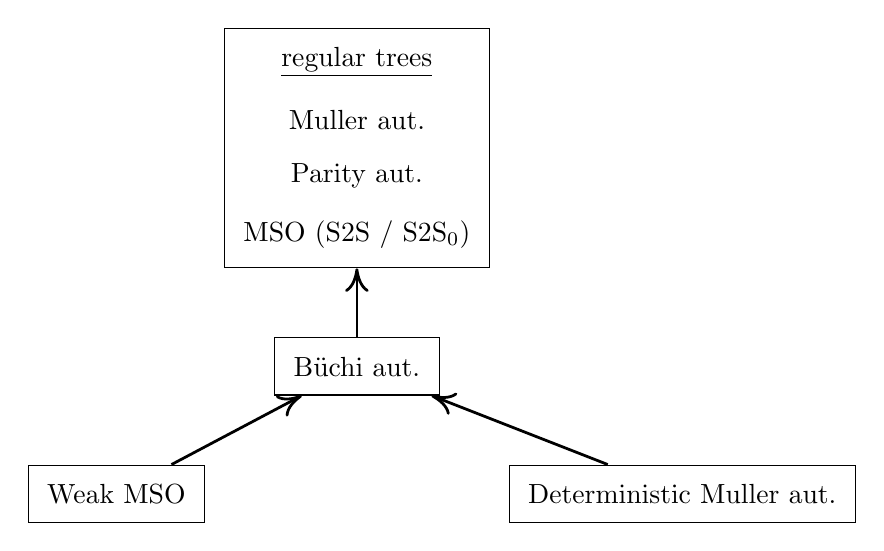
\begin{tikzpicture}
  \node (ireg) {\underline{regular trees}};
  \node (iMTA) [below=5pt of ireg] {Muller aut.};
  \node (iPTA) [below=5pt of iMTA] {Parity aut.};
  \node (iMSO) [below=5pt of iPTA] {MSO (S2S / S2S\textsubscript{0})};
  \node [draw, fit={(ireg) (iMTA) (iPTA) (iMSO)}] (c1) {};
  
  \node (iBTA) [below=of c1] {Büchi aut.};
  \node [draw, fit={(iBTA)}] (c2) {};
  
  \node (iWMSO) [below left=of c2] {Weak MSO};
  \node [draw, fit={(iWMSO)}] (c3) {};
  
  \node (iDMTA) [below right=of c2] {Deterministic Muller aut.};
  \node [draw, fit={(iDMTA)}] (c4) {};
  
  \draw [-{>[length=3mm,width=3mm]}, line width=1pt] (c2) -- (c1);
  \draw [-{>[length=3mm,width=3mm]}, line width=1pt] (c3) -- (c2);
  \draw [-{>[length=3mm,width=3mm]}, line width=1pt] (c4) -- (c2);
\end{tikzpicture}

\subsection{Class Differences}
TODO

\subsection{Class Equalities}
TODO

\subsection{Closures}
TODO


\end{document}
















